\documentclass[11pt,a4paper]{ctexart}
\usepackage[margin=2.2cm]{geometry}
\usepackage{amsmath,amssymb,booktabs,longtable,graphicx,float,array,xcolor,hyperref}
\hypersetup{colorlinks=true,linkcolor=blue,urlcolor=blue}
\setlength{\parindent}{2em}
\setlength{\parskip}{0.35em}
\title{第四次作业：一维 $J_1$--$J_2$ XXZ 自旋链的对称性分块精确对角化}
\author{}
\date{\today}

\begin{document}
\maketitle

\begin{abstract}
本文在固定总磁量子数 $S^z_{\rm tot}$ 的 $U(1)$ 扇区内进一步利用平移对称性，完成周期边界自旋 $1/2$ $J_1$--$J_2$ XXZ 链的精确对角化。主计算采用 $N=16,J_1=1,\Delta=1$，比较 $J_2=0$ 与 Majumdar--Ghosh 点 $J_2=0.5$。除必做的基态、动量分块全谱、局域磁矩和磁化曲线外，还计算 XX 自由费米子基准、关联函数与结构因子、$J_2$ 扫描和两种能隙。全部 57 项独立校验及故障注入测试均通过。
\end{abstract}

\section{模型与基}
哈密顿量为
\begin{align}
H={}&J_1\sum_j\left(S_j^xS_{j+1}^x+S_j^yS_{j+1}^y+\Delta S_j^zS_{j+1}^z\right)\\
&+J_2\sum_j\left(S_j^xS_{j+2}^x+S_j^yS_{j+2}^y+\Delta S_j^zS_{j+2}^z\right).
\end{align}
位 $j$ 表示格点 $j$，1 表示自旋向上。固定 $n_\uparrow$ 后，$S^z_{\rm tot}=n_\uparrow-N/2$，基维数为 $\binom{N}{n_\uparrow}$。对一条键 $(i,j)$，纵向项贡献 $\pm J\Delta/4$，横向项在两自旋反平行时翻转二者并给出矩阵元 $J/2$。$N=2$ 的最近邻物理键只计一次。

\subsection{平移与费米符号说明}
平移定义为把格点 $j$ 的自旋移到 $j+1$。当前基是自旋张量积基而非费米 Fock 基，因此 $T$ 是非零元全为 $+1$ 的纯置换矩阵，位串跨越边界时不附加费米交换负号。费米奇偶性仅在第\ref{sec:xx}节 Jordan--Wigner 解析映射的边界条件中出现。

设平移轨道长度为 $\ell$，采用
\begin{equation}
|r;k\rangle=\frac1{\sqrt\ell}\sum_{n=0}^{\ell-1}e^{-ikn}T^n|r\rangle,
\qquad k=\frac{2\pi m}{N}.
\end{equation}
只有 $e^{ik\ell}=1$ 时该列非零，并有 $T|r;k\rangle=e^{ik}|r;k\rangle$。最终分块为 $H_k=P_k^\dagger HP_k$。

\section{维数与基态}
$N=16,S^z_{\rm tot}=0$ 的维数为 $\binom{16}{8}=12870$；所有磁量子数扇区维数之和为 $65536=2^{16}$。
\begin{table}[H]
\centering
\caption{$N=16$ 基态结果。}
\begin{tabular}{ccccc}
\toprule
$J_2$ & $E_0$ & $E_0/N$ & 简并度 & 基态 $m$ \\
\midrule
0 & -7.142296360617 & -0.446393522539 & 1 & 0 \\
0.5 & -6.000000000000 & -0.375000000000 & 2 & 0,8 \\
\bottomrule
\end{tabular}
\end{table}
其中 $k=2\pi m/16$。$J_2=0.5$ 的能量精确满足 $E_0=-3N/8=-6$，两个基态分别位于 $k=0,\pi$。

\section{动量分块与最低激发}
\begin{longtable}{rrrrr}
\caption{$N=16$ 的动量块维数与最低能量。}\\
\toprule
$m$ & $k/\pi$ & 维数 & $E_0(k),J_2=0$ & $E_0(k),J_2=0.5$\\
\midrule
\endfirsthead
\toprule
$m$ & $k/\pi$ & 维数 & $E_0(k),J_2=0$ & $E_0(k),J_2=0.5$\\
\midrule
\endhead
0&0.000&810&-7.142296361&-6.000000000\\
1&0.125&800&-6.523407057&-5.655208935\\
2&0.250&808&-5.990986863&-5.452760304\\
3&0.375&800&-5.615175598&-5.195284120\\
4&0.500&809&-5.451965668&-5.000000000\\
5&0.625&800&-5.525353087&-5.183968217\\
6&0.750&808&-5.823231143&-5.470824884\\
7&0.875&800&-6.298652725&-5.610665883\\
8&1.000&810&-6.872106678&-6.000000000\\
9&1.125&800&-6.298652725&-5.610665883\\
10&1.250&808&-5.823231143&-5.470824884\\
11&1.375&800&-5.525353087&-5.183968217\\
12&1.500&809&-5.451965668&-5.000000000\\
13&1.625&800&-5.615175598&-5.195284120\\
14&1.750&808&-5.990986863&-5.452760304\\
15&1.875&800&-6.523407057&-5.655208935\\
\bottomrule
\end{longtable}
块维数之和为 12870。两种参数下去除基态流形后的最低激发都在 $m=8$。对应能隙分别为 0.270189682250 和 0.285717141070。
\begin{figure}[H]
\centering
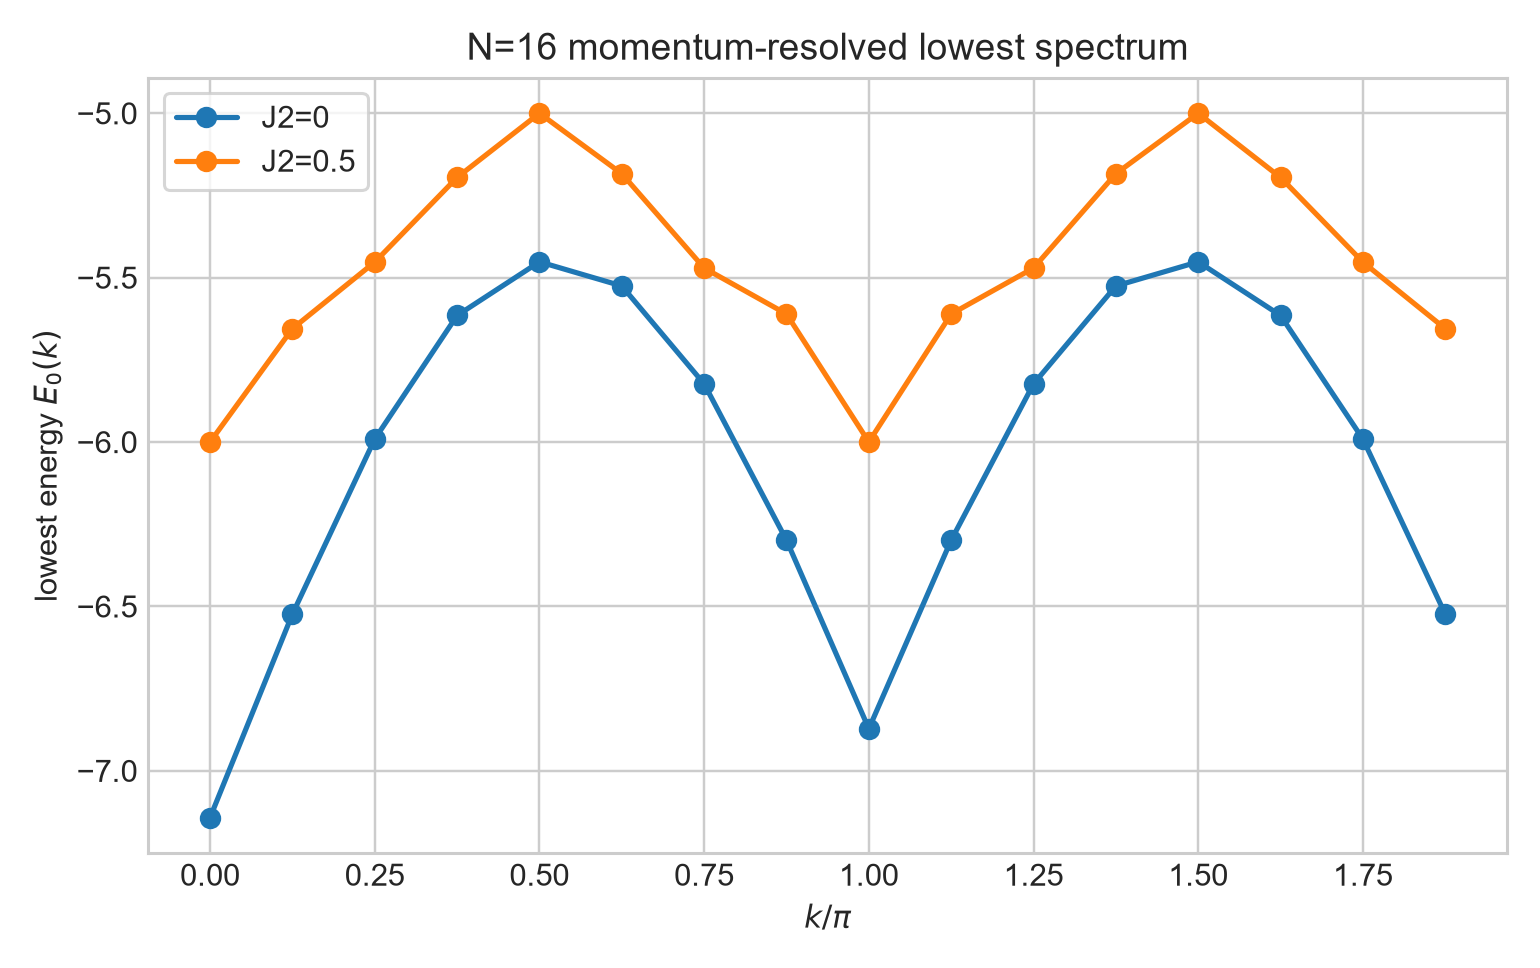
\includegraphics[width=0.82\linewidth]{figures/dispersion_n16.png}
\caption{$N=16$ 各动量块最低能量。}
\end{figure}
\subsection{$N=8$ 各动量块全谱}
下列各行按能量升序列出该动量块的全部本征值。

{\small
\begin{longtable}{c>{\raggedright\arraybackslash}p{13.2cm}}
\caption{$N=8,J_2=0$ 的完整动量分块谱。}\\
\toprule
$m$ & 全部本征值\\
\midrule
\endfirsthead
\toprule
$m$ & 全部本征值\\
\midrule
\endhead
0 & -3.651093409, -1.801937736, -1.000000000, -0.726109445, -0.445041868, 0, 0, 0.377202854, 1.246979604, 2.000000000\\
1 & -2.458738509, -1.144122806, -0.628378427, -0.512683203, -0.292893219, 0.437016024, 0.892693358, 1.707106781\\
2 & -1.854637680, -1.618033989, -1.267035098, -0.596968283, -0.258652023, 0.451605963, 0.618033989, 1.000000000, 1.525687121\\
3 & -2.145148374, -1.707106781, -0.858923550, -0.437016024, 0.265452712, 0.292893219, 1.144122806, 1.445725993\\
4 & -3.128419064, -2.699628148, -1.201639676, -0.760876722, 0, 0, 0, 1.000000000, 1.330058740, 1.460504870\\
5 & -2.145148374, -1.707106781, -0.858923550, -0.437016024, 0.265452712, 0.292893219, 1.144122806, 1.445725993\\
6 & -1.854637680, -1.618033989, -1.267035098, -0.596968283, -0.258652023, 0.451605963, 0.618033989, 1.000000000, 1.525687121\\
7 & -2.458738509, -1.144122806, -0.628378427, -0.512683203, -0.292893219, 0.437016024, 0.892693358, 1.707106781\\
\bottomrule
\end{longtable}

\begin{longtable}{c>{\raggedright\arraybackslash}p{13.2cm}}
\caption{$N=8,J_2=0.5$ 的完整动量分块谱。}\\
\toprule
$m$ & 全部本征值\\
\midrule
\endfirsthead
\toprule
$m$ & 全部本征值\\
\midrule
\endhead
0 & -3.000000000, -2.000000000, -1.707106781, -1.224744871, -0.500000000, -0.500000000, -0.292893219, 0, 1.224744871, 3.000000000\\
1 & -2.438379908, -1.113315380, -0.965925826, -0.792893219, -0.711249716, 0.258819045, 0.555838223, 2.207106781\\
2 & -2.000000000, -2.000000000, -1.500000000, -1.186140662, 0, 0, 0, 1.000000000, 1.686140662\\
3 & -2.207106781, -2.054647409, -1.271985559, -0.384841784, -0.258819045, 0.792893219, 0.965925826, 1.418581533\\
4 & -3.000000000, -2.595483037, -1.414213562, -1.072282878, -0.707106781, -0.500000000, 0.707106781, 1.000000000, 1.167765915, 1.414213562\\
5 & -2.207106781, -2.054647409, -1.271985559, -0.384841784, -0.258819045, 0.792893219, 0.965925826, 1.418581533\\
6 & -2.000000000, -2.000000000, -1.500000000, -1.186140662, 0, 0, 0, 1.000000000, 1.686140662\\
7 & -2.438379908, -1.113315380, -0.965925826, -0.792893219, -0.711249716, 0.258819045, 0.555838223, 2.207106781\\
\bottomrule
\end{longtable}
}
两组谱并集与直接 $S^z_{\rm tot}=0$ 谱的最大误差分别为 $5.77\times10^{-15}$ 与 $5.55\times10^{-15}$，完整精度数据同时保存在随附 CSV 中。

\section{局域磁矩与磁化}
在简并基态空间内先对角化平移算符，再选择确定动量态。两组参数均有
\begin{equation}
\max_i|\langle S_i^z\rangle|<5.4\times10^{-15},\qquad
\max_i|\langle S_i^x\rangle|=0.
\end{equation}
这正是有限尺寸 $SU(2)$ 单态的结果。为得到非平凡磁化响应，对全部 $M=S^z_{\rm tot}$ 求 $E_0(M)$ 并取 $E_0(M)-hM$ 的下包络。
\begin{table}[H]
\centering
\caption{正磁场下的临界场。}
\begin{tabular}{ccc}
\toprule
跃迁 & $J_2=0$ & $J_2=0.5$\\
\midrule
$0\to1$&0.270189682&0.285717141\\
$1\to2$&0.749791411&0.587317531\\
$2\to3$&1.147732172&1.064623952\\
$3\to4$&1.462448409&1.670145424\\
$4\to5$&1.697133062&1.926229829\\
$5\to6$&1.858706422&2.042732244\\
$6\to7$&1.956295201&2.186997056\\
$7\to8$&2.000000000&2.236236823\\
\bottomrule
\end{tabular}
\end{table}
\begin{figure}[H]
\centering
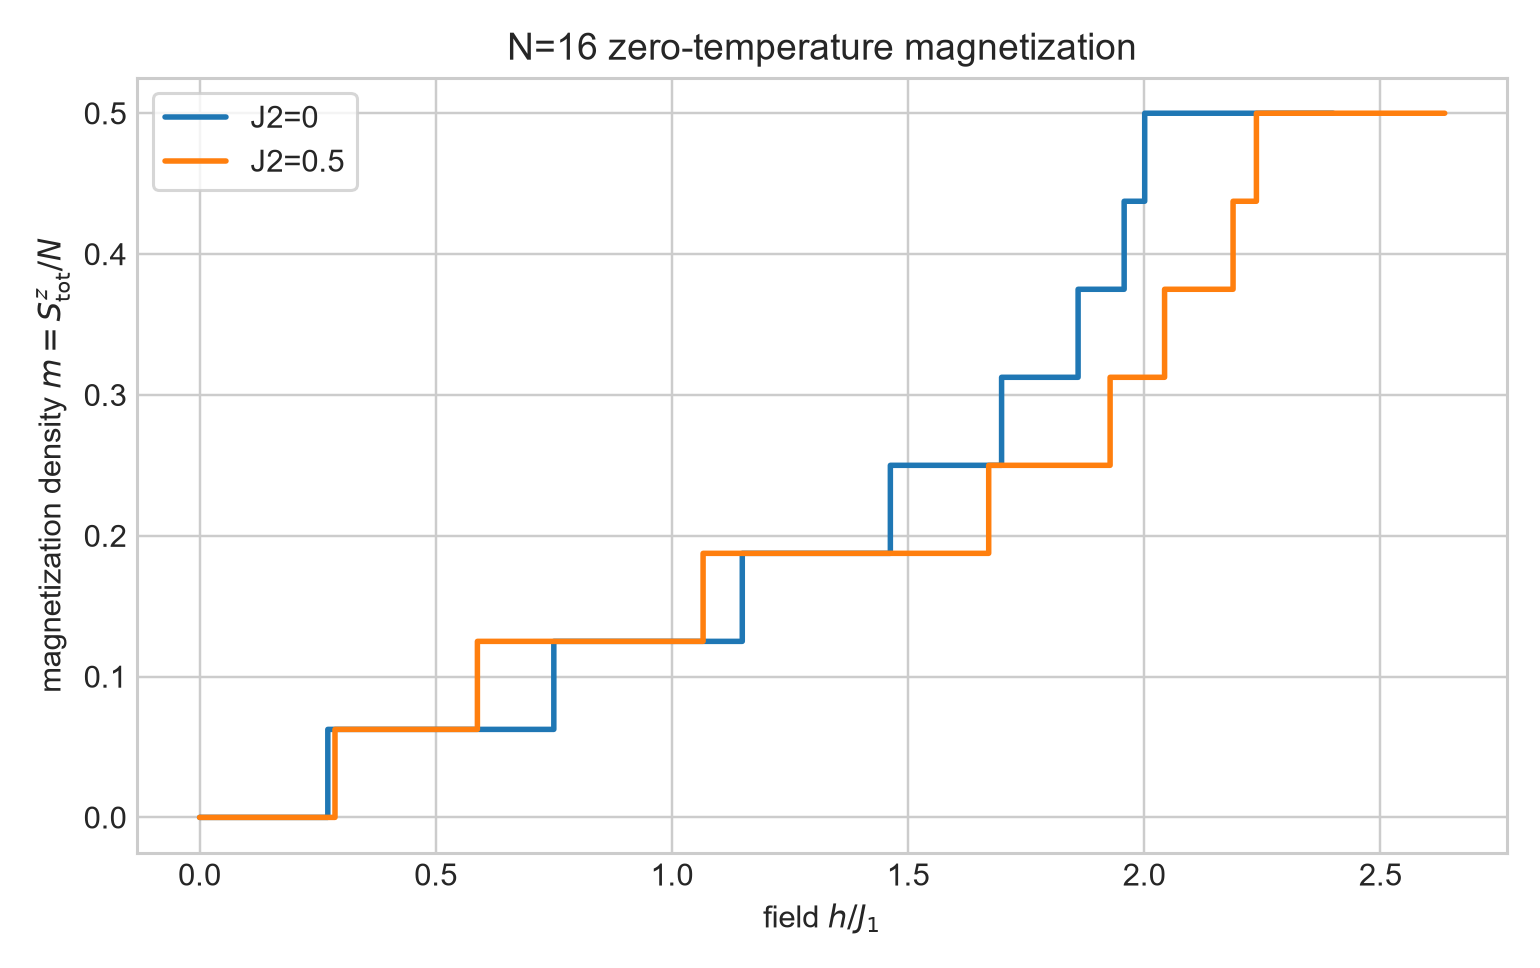
\includegraphics[width=0.82\linewidth]{figures/magnetization_n16.png}
\caption{$N=16$ 零温磁化密度。}
\end{figure}

\section{Majumdar--Ghosh 精确态}
以 $|s_{ab}\rangle=(|\uparrow_a\downarrow_b\rangle-|\downarrow_a\uparrow_b\rangle)/\sqrt2$ 构造 $D_0,D_1$。结果如下。
\begin{table}[H]
\centering
\caption{较大体系 ED 基态能量与解析值。}
\begin{tabular}{cccc}
\toprule
$N$ & ED 基态能量 & $-3N/8$ & 绝对差\\
\midrule
10 & -3.750000000000 & -3.750000000000 & $2.67\times10^{-15}$\\
12 & -4.500000000000 & -4.500000000000 & $5.33\times10^{-15}$\\
\bottomrule
\end{tabular}
\end{table}
\begin{table}[H]
\centering
\begin{tabular}{ccccc}
\toprule
$N$ & $-3N/8$ & $\|(H-E)D_0\|$ & $\|(H-E)D_1\|$ & $\langle D_0|D_1\rangle$\\
\midrule
8&-3.00&0&0&0.125000\\
10&-3.75&$2.72\times10^{-16}$&$2.72\times10^{-16}$&-0.062500\\
12&-4.50&$5.21\times10^{-16}$&$5.21\times10^{-16}$&0.031250\\
\bottomrule
\end{tabular}
\end{table}
$D_0,D_1$ 单独不是平移本征态，但 $TD_0=D_1$；归一化 $D_0\pm D_1$ 分别是 $k=0,\pi$ 态，平移残差为零。

\section{关联、结构因子与能隙}
计算
\begin{equation}
C(r)=\langle\mathbf S_0\cdot\mathbf S_r\rangle,
\qquad S(q)=\frac1N\sum_re^{-iqr}C(r).
\end{equation}
对离散动量 $q=2\pi n/N$，该归一化给出独立求和规则
\begin{equation}
\sum_qS(q)=\frac1N\sum_rC(r)\sum_qe^{-iqr}=C(0)=\frac34.
\end{equation}
两组数据对该规则的误差均小于 $2\times10^{-16}$。此外，$\Delta=1$ 时 $\sum_rC(r)$ 残差小于 $8\times10^{-16}$，且逐点满足 $C(r)=3\langle S_0^zS_r^z\rangle$，最大误差小于 $2\times10^{-14}$。改为 $\Delta=0.5$ 后最大偏差为 0.106711105，显示 $SU(2)$ 破缺。结构因子峰值均在 $q=\pi$。
\begin{figure}[H]
\centering
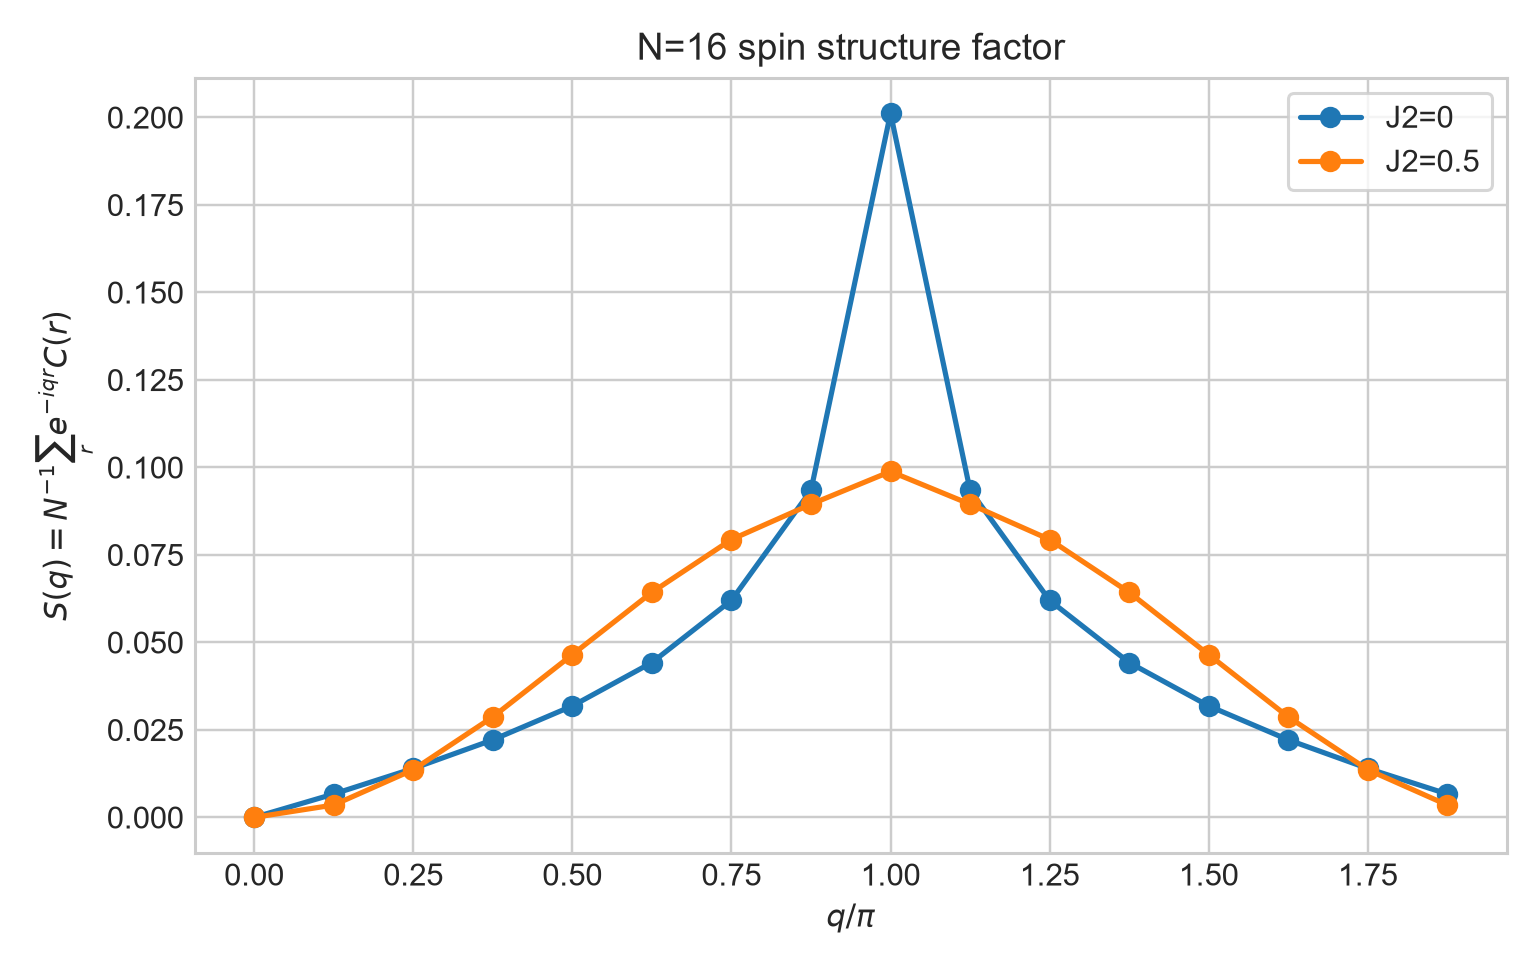
\includegraphics[width=0.82\linewidth]{figures/structure_factor_n16.png}
\caption{$N=16$ 自旋结构因子。}
\end{figure}
有限尺寸自旋隙分别为 0.270189682250 与 0.285717141070；最低 $S^z_{\rm tot}=0$ 非基态激发隙在数值精度内相同。

\section{XX 自由费米子基准}\label{sec:xx}
$\Delta=0$ 时 $\epsilon(k)=J_1\cos k$。分别测试周期和反周期 Jordan--Wigner 动量格点：
\begin{table}[H]
\centering
\begin{tabular}{ccccc}
\toprule
$N$ & 自旋数值 & 自由费米子 & 边界 & 误差\\
\midrule
8&-2.613125929753&-2.613125929753&反周期&$1.33\times10^{-15}$\\
10&-3.236067977500&-3.236067977500&周期&$1.78\times10^{-15}$\\
12&-3.863703305156&-3.863703305156&反周期&$2.66\times10^{-15}$\\
\bottomrule
\end{tabular}
\end{table}
$N=8$ 若错误采用周期边界，能量偏差达到 0.198912367，明确定位了费米符号应出现的位置。

\section{$J_2$ 扫描}
\begin{figure}[H]
\centering
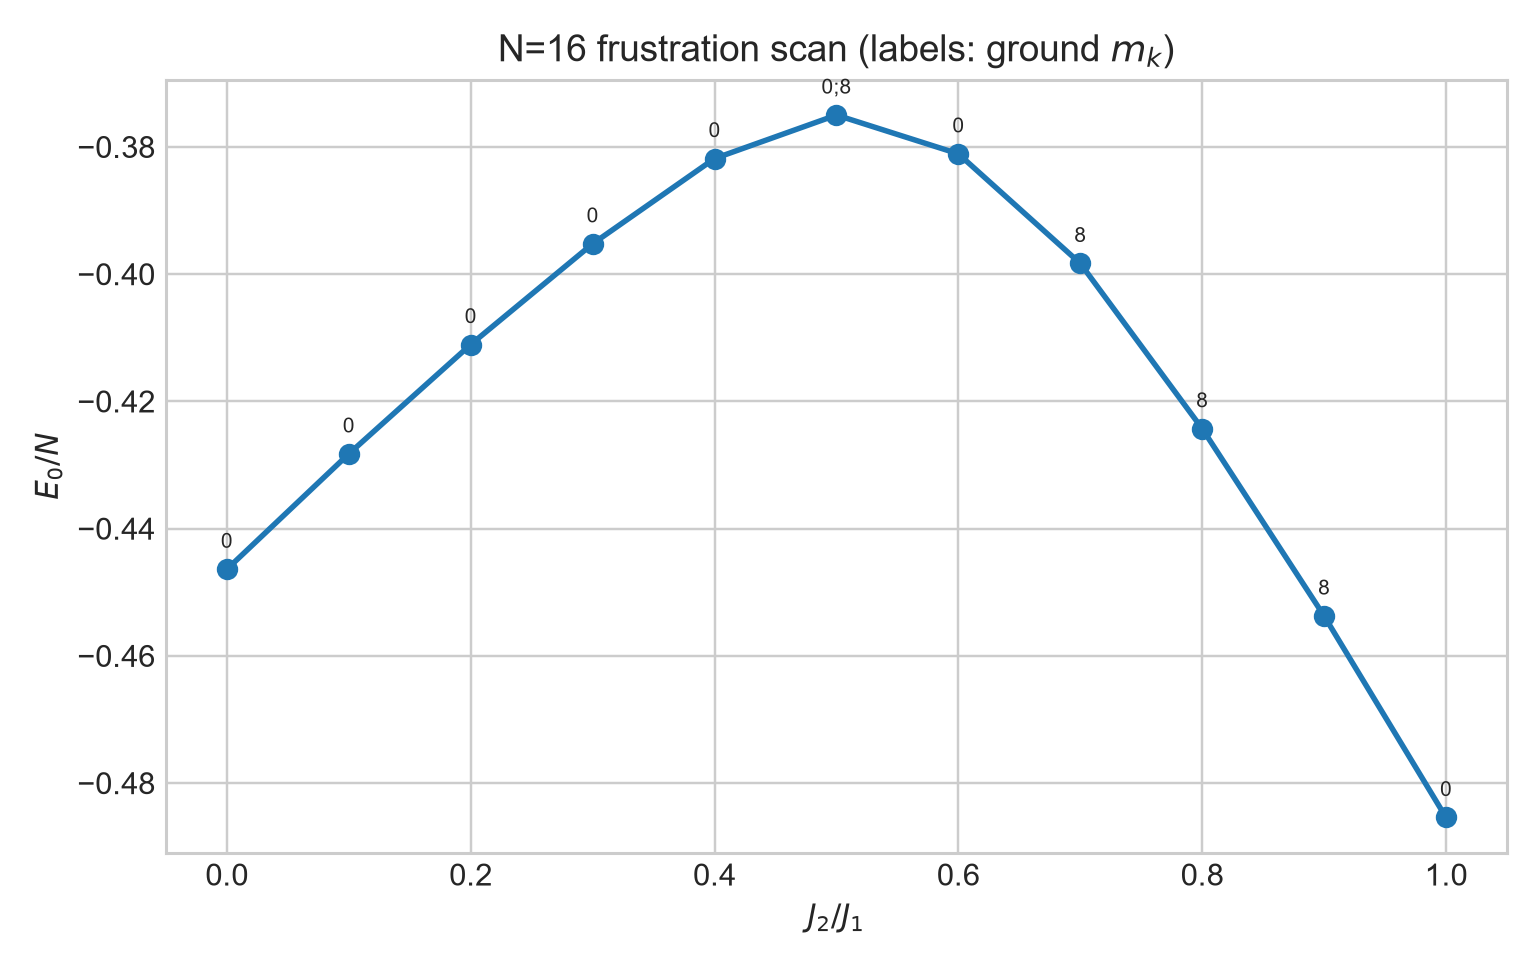
\includegraphics[width=0.82\linewidth]{figures/j2_scan_n16.png}
\caption{$J_2/J_1=0,0.1,\ldots,1.0$ 的基态能量；标注为动量指标 $m$。}
\end{figure}
在 $J_2=0.5$ 出现 $m=0,8$ 精确简并，这是 Majumdar--Ghosh 精确二聚体点。另一方面，$J_2=0.6$ 时最低态为 $m=0$，$J_2=0.7$ 时变为 $m=8$，所以步长 0.1 的扫描还把另一次动量扇区能级交叉夹在二者之间，中点约为 0.65。这个 0.65 只是 $N=16$ 与当前扫描分辨率下的有限尺寸交叉位置，不能与精确二聚体点 0.5 等同，也不能直接视为热力学极限相变点。$J_2=1.0$ 时基态又回到 $m=0$，进一步说明有限环会出现多次离散动量能级交叉。

\section{验证与故障注入}
57 项检查全部通过。表\ref{tab:validation-intent} 显式说明每类校检针对的错误及错误时的失败方式；同一机制在不同 $J_2$ 或 $N$ 上重复执行的每一条独立记录，均在随附 \texttt{validation\_checks.csv} 中带有 \texttt{targeted\_error} 和 \texttt{failure\_signature} 字段。

{\scriptsize
\begin{longtable}{>{\raggedright\arraybackslash}p{2.2cm}>{\raggedright\arraybackslash}p{4.1cm}>{\raggedright\arraybackslash}p{5.2cm}>{\raggedright\arraybackslash}p{2.6cm}}
\caption{校检所针对的错误、预期失败方式与实测。}\label{tab:validation-intent}\\
\toprule
校检 & 针对的错误 & 实现错误时的失败方式 & 本次实测\\
\midrule
\endfirsthead
\toprule
校检 & 针对的错误 & 实现错误时的失败方式 & 本次实测\\
\midrule
\endhead
扇区维数 & popcount 漏态、重复态或 $S^z$ 换算错误 & 维数和不等于 $2^{16}$，零磁化维数偏离 $\binom{16}{8}$ & 65536；12870\\
$N=2,4$ 精确谱 & 键双计数、XY 系数或 $S^zS^z$ 符号错误 & $N=2$ 偏离 $-3/4,+1/4$；$N=4$ 偏离 $-2$ & 最大误差 $2.22\times10^{-16}$\\
平移置换与 $T^N$ & 错加费米负号、位旋转或边界掩码错误 & $T$ 出现 $-1$；某个位串平移 $N$ 次不返回自身 & 两项残差均为 0\\
$H=H^\dagger,[H,T]=0$ & 单向跃迁、共轭索引、周期键编号错误 & $H-H^\dagger$ 或 $HT-TH$ 出现非零元 & 两组均为 0\\
$P_k^\dagger P_k=I$ & 轨道重复、短轨道条件或 $1/\sqrt\ell$ 错误 & Gram 矩阵非单位阵；漏归一化时对角元放大 & $2.22\times10^{-16}$\\
$TP_k=e^{ik}P_k$ & 指数正负号或平移方向错误 & 残差非零，常把 $m$ 错标为 $N-m$ & $2.64\times10^{-15}$\\
块维数与基态一致性 & 动量态漏/重或 $P_k^\dagger HP_k$ 装配错误 & 块维数和不等于 12870，块最低值不等于 U(1) 基态 & 能量最大差 $3.11\times10^{-14}$\\
局域磁矩规则 & bit 自旋约定、局域算符或扇区重构错误 & $\sum_i\langle S_i^z\rangle\ne0$，或固定扇区出现 $\langle S_i^x\rangle\ne0$ & $1.75\times10^{-16}$；0\\
关联与结构因子 & 横向关联系数或 $1/N$ 归一化错误 & $\sum_rC(r)\ne0$；$\sum_qS(q)\ne3/4$，漏 $1/N$ 时得到 12 & $7.77\times10^{-16}$；0.75\\
$SU(2)$ 与各向异性对照 & 点积关联系数错，或 $\Delta$ 被硬编码 & $\Delta=1$ 时 $C-3C_{zz}\ne0$；$\Delta=0.5$ 时又错误为 0 & $1.90\times10^{-14}$；0.106711105\\
自旋反演 & 上下自旋编码或扇区构造不对称 & $E(M)\ne E(-M)$ & $8.88\times10^{-15}$\\
$N=8$ 谱并集 & 动量轨道漏/重或块谱未求全 & 70 个拼接能级不能逐点匹配直接 U(1) 谱 & 最大 $5.77\times10^{-15}$\\
MG 残差、能量、动量 & $J_2$ 系数、二聚体符号或平移组合错误 & $(H+3N/8)D\ne0$、ED 偏离 $-3N/8$ 或 $T\psi\ne\pm\psi$ & 最大 $5.33\times10^{-15}$\\
XX 自由费米子 & XY 幅度、JW 奇偶边界或占据规则错误 & 自旋 ED 与正确周期/反周期填充能量不符 & 最大 $4.00\times10^{-15}$\\
\bottomrule
\end{longtable}
}

为验证这些校检确实有检错力，又注入四类故障：$N=2$ 键双计数使 $E_0$ 从 $-0.75$ 变为 $-1.5$；漏掉投影归一化使 Gram 偏差变为 15；$J_2=0.5$ 漏掉次近邻键使能量错成 $-7.142296361$ 而非 $-6$；$N=8$ XX 选错边界产生 0.198912367 的能量偏差。四种错误均按表中预期方式失败并被捕获。

\section{结论}
固定 $U(1)$ 扇区与平移动量的联合分块把 $N=16$ 的 12870 维零磁化空间拆为约 800 维的块，同时保留了完整物理信息。结果正确再现 Heisenberg 基准、Majumdar--Ghosh 双重基态与 XX 自由费米子极限；磁化下包络、关联函数和能隙提供了比局域零磁矩更完整的有限尺寸物理解读。特别地，自旋平移不含额外费米负号，而 Jordan--Wigner 边界奇偶性必须仅在自由费米子映射中处理。

\end{document}
